\documentclass{report}
\usepackage{graphicx}
\graphicspath{ {./images/} }

\begin{document}

\title{LCOM Final Report}
	\author{Eduardo da Costa Correia\\
	\texttt{up201806433}
	\and
	Tiago Duarte Silva\\
	\texttt{up201806516}}   
\maketitle

\tableofcontents

\chapter{Instruções de Utilização} 

\section{Menu Principal}

Ao iniciar o programa, é apresentada o menu principal, onde o jogador pode selecionar um dos dois modos de jogos possíveis, cada um com a opção de se jogar ou não com outro jogador.

\begin{itemize}
	\item Campaign

	\begin{itemize}
		\item Singleplayer 
		\item Co-Op
	\end{itemize}
	
	\item Arcade
	
	\begin{itemize}
		\item Singleplayer 
		\item Versus
	\end{itemize}
\end{itemize}

Para sair do jogo, o utilizador deve pressionar \textit{Esc} duas vezes, o mesmo para voltar ao menu principal a partir de um dos modos de jogo.

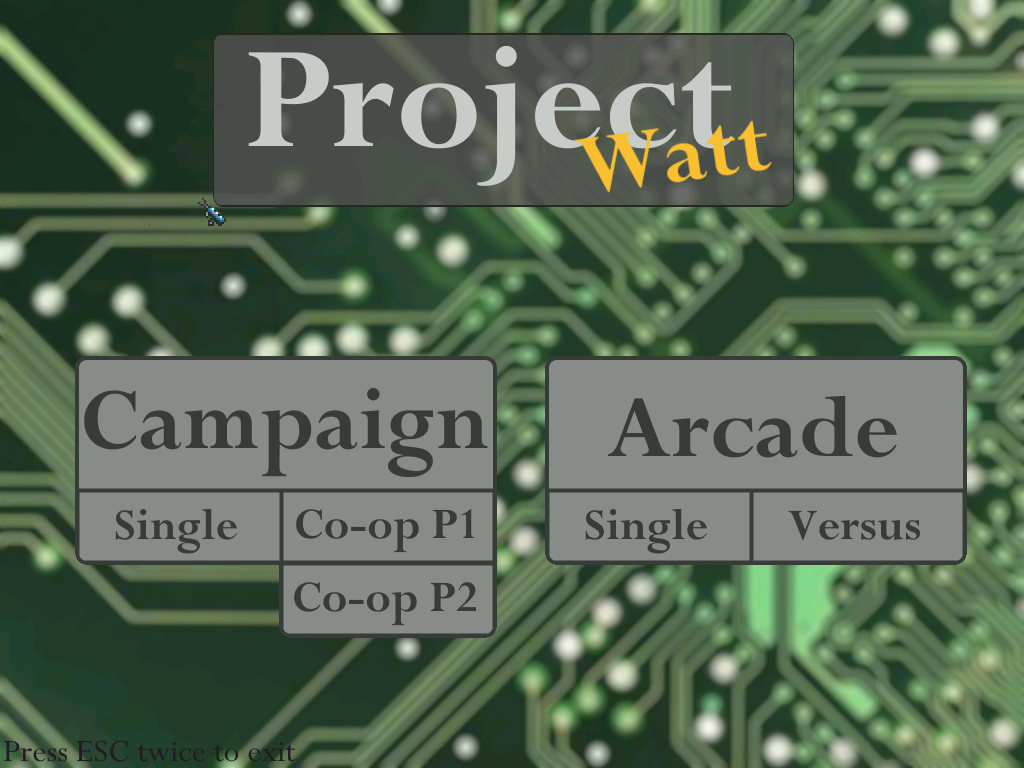
\includegraphics[width=\textwidth]{main_menu}

\section{Campaign}

Este é o modo de jogo \textit{principal} em que um jogador controla a personagem \textit{Watt}, uma faísca que ficou "presa" num curto-circuito e que para sair terá de fazer "ligação à terra", ou seja, neste caso, a personagem tem de alcançar o canto superior direito do mapa. Para isso tem de ultrapassar diversos obstáculos tais como os espinhos e lasers (se tocar num destes a faísca dissipa-se e volta ao início). \newline
O movimento da personagem principal é controlado pelas teclas W, A, S, D ou pelas setas $\uparrow$, $\leftarrow$, $\downarrow$ e $\rightarrow$ e o seu salto pela tecla Z ou pelo Espaço.
Para além disso, é possível controlar certos aspetos da jogabilidade, como a altura do salto da personagem e a sua velocidade (através dos \textit{sliders} azul e laranja respetivamente), qual dos lasers está inativo (vermelho, azul ou roxo - através dos botões com a cor correspondente) e o sentido da gravidade da personagem (através da tecla X em multiplayer, uma knob em Co-Op). Todos estes aspetos são controlados pelo segundo jogador se estiver a jogar em Co-Op.

\includegraphics[width=\textwidth]{singleplayer}

\section{Arcade}

Um modo de jogo alternativo, baseado na mecânica de anti-gravidade do outro modo de jogo, em que o jogador terá de se desviar de lasers que vêm na sua direção, passando por entre estes e tentanto aguentar o máximo de tempo possível sem tocar neles e perder.

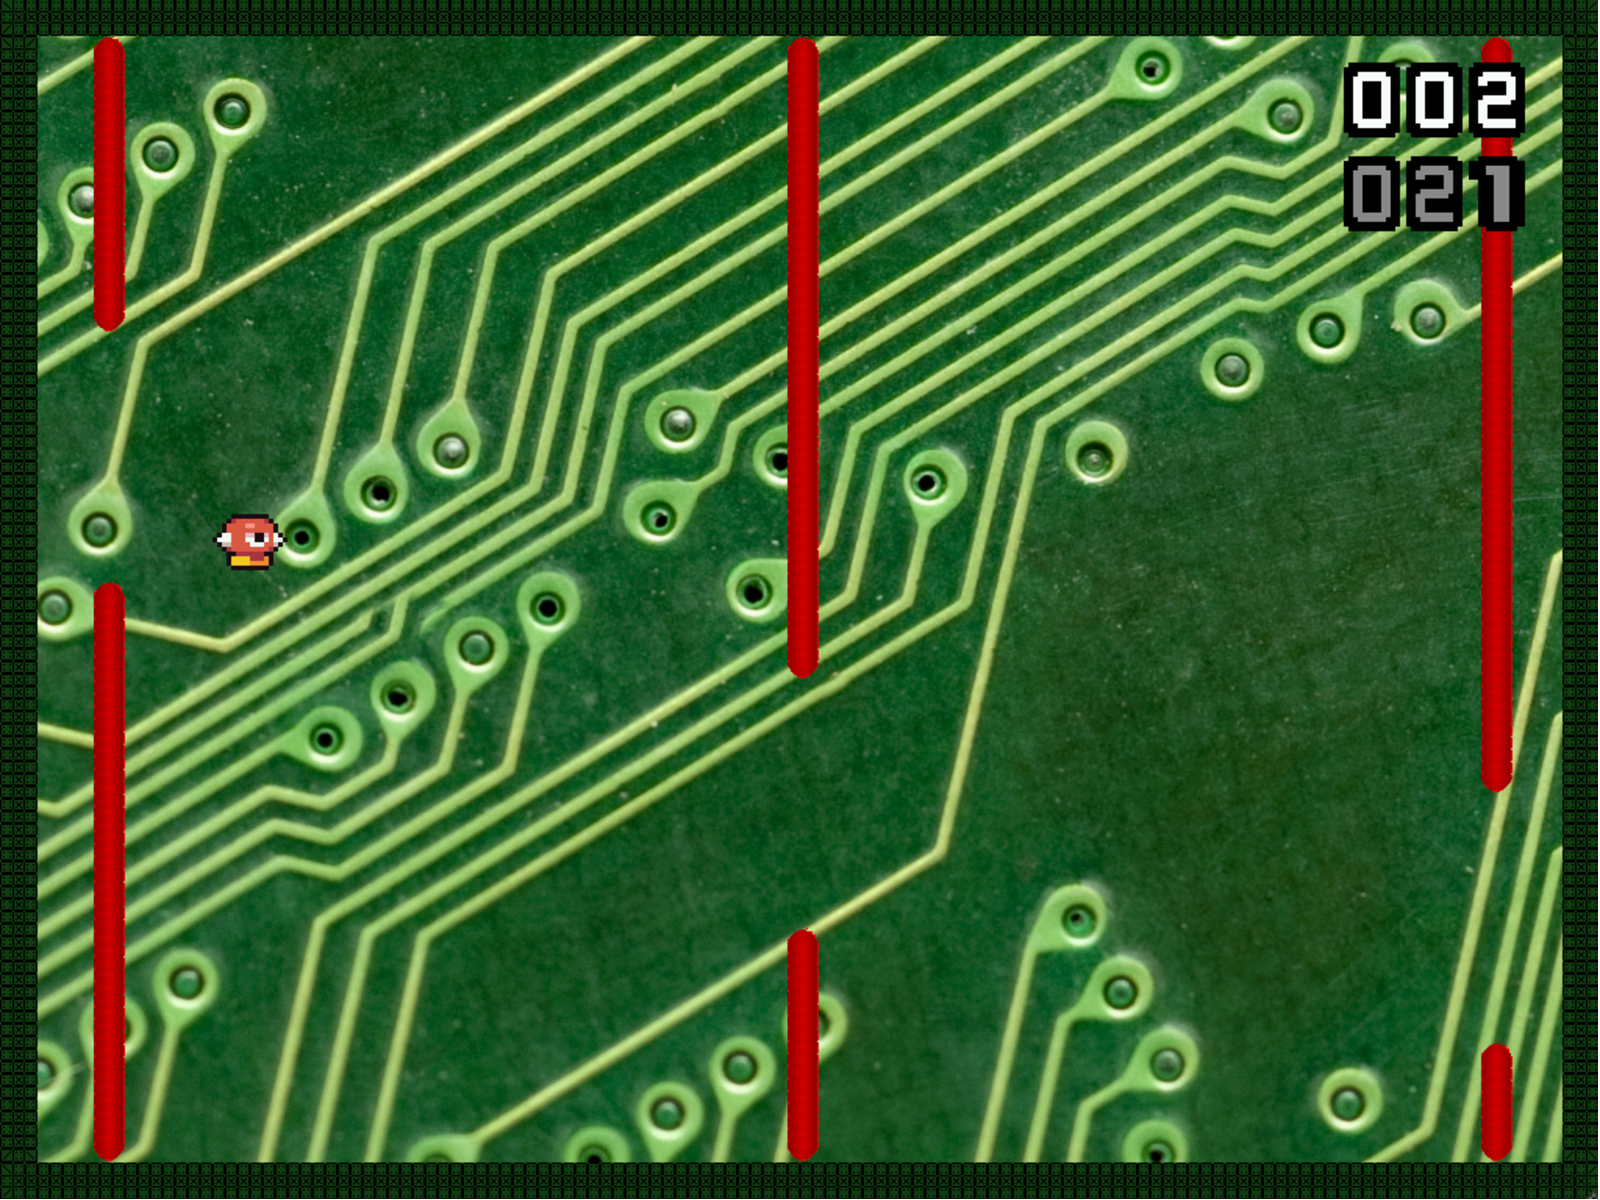
\includegraphics[width=\textwidth]{arcade}

\chapter{Estado do Projeto}

\section{Dispositivos Usados}

\begin{center}
	\begin{tabular}{ |c|c|c| } 
		\hline
			Dispositivo & Utilização & Interrupção \\ 
		\hline
		\hline
			Timer & N/A & Sim \\ 
			Teclado & Controlo da personagem 1 & Sim \\ 
			Rato & Menus e personagem 2 & Sim\\
			Placa Gráfica & N/A & Não\\
			Real Time Clock & Efeito temporário & Sim\\
			Serial Port & N/A & Sim \\
		\hline
	\end{tabular}
\end{center}

\subsection{Timer}

Framerate handling

\subsection{Teclado}

\subsection{Rato}

Usado no menu principal para selecionar o modo de jogo e para controlar sliders/knob.

\subsection{Placa Gráfica}

RGB 565

\subsection{Real Time Clock}

\subsection{Serial Port}

Usado nos modos multiplayer (Campaign - Co-Op e Arcade - Versus). No primeiro, as personagens 1 e 2 seriam controladas pelos utilizadores em máquinas separadas 

\chapter{Organização e Estrutura do Código}

\chapter{Detalhes de Implementação}

\chapter{Conclusões}

\end{document}